\section{Affichage d'une ligne grace au CPU :}
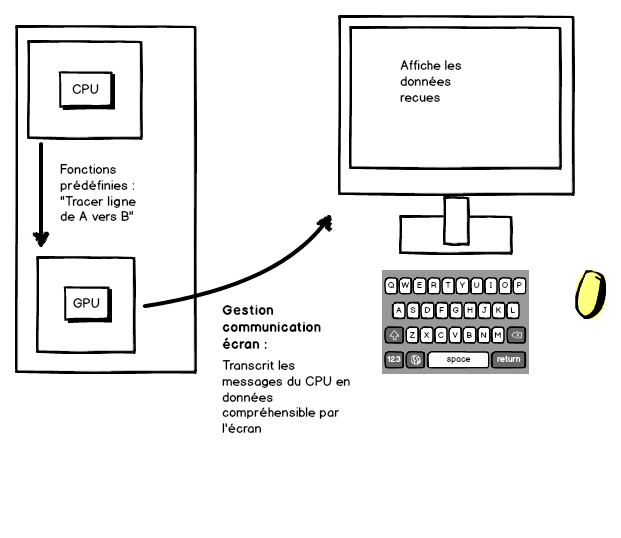
\includegraphics[width=12cm,height=9cm]{img/cpuRaster.png} \\
Dans ce cas le CPU (Unité central de calcul) va effectuer tout les calculs matriciels lui même et les envoyer à la carte graphique. Voir l'exemple ci-dessous.
\subsection{Exemple :}
\begin{center}
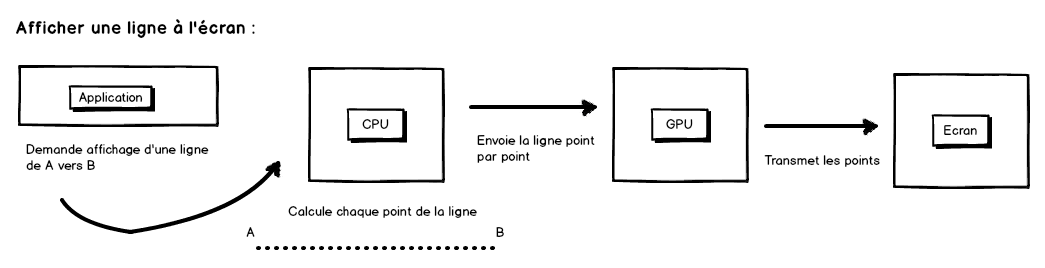
\includegraphics[width=15cm,height=4cm]{img/cpuRasterExemple.png}
\end{center}
C'est donc le CPU qui va effectuer la demande de l'application en transformant cette ligne en plusieurs petits points qui seront envoyés un par un au GPU. Lui les envera sous forme de pixel à l'écran.\\
Cela est très lourd pour le CPU. Son architecture n'étant faite que de quelque coeur puissant, celui ci n'est pas otpimisé pour effectuer de nombreux de calcul en peu de temps. L'optimisation serai donc de parraléliser ces calculs... L'utilisation d'une unité graphique de calcul devient interessante.

\section{Affichage d'une ligne grace au GPU :}
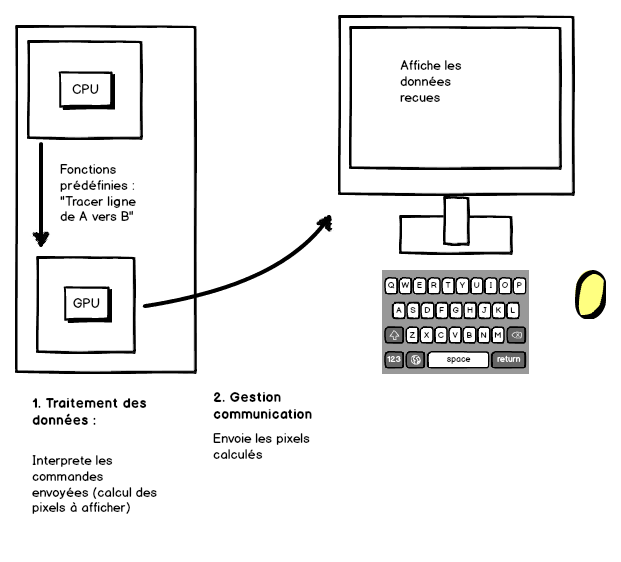
\includegraphics[width=12cm,height=10cm]{img/gpuRaster.png} \\
Maintenant le CPU n'a qu'à transcrire la demande faite par l'application à son pilote graphique. Celui-ci s'occupe d'envoyer la requête au GPU (Unité graphique de calcul) qui effectuera les calculs matriciels. Pour communiquer facillement avec ce pilote on utilise traditionnellement des API (exemple : OpenGL ou DirectX).
\subsection{Exemple :}
\begin{center}
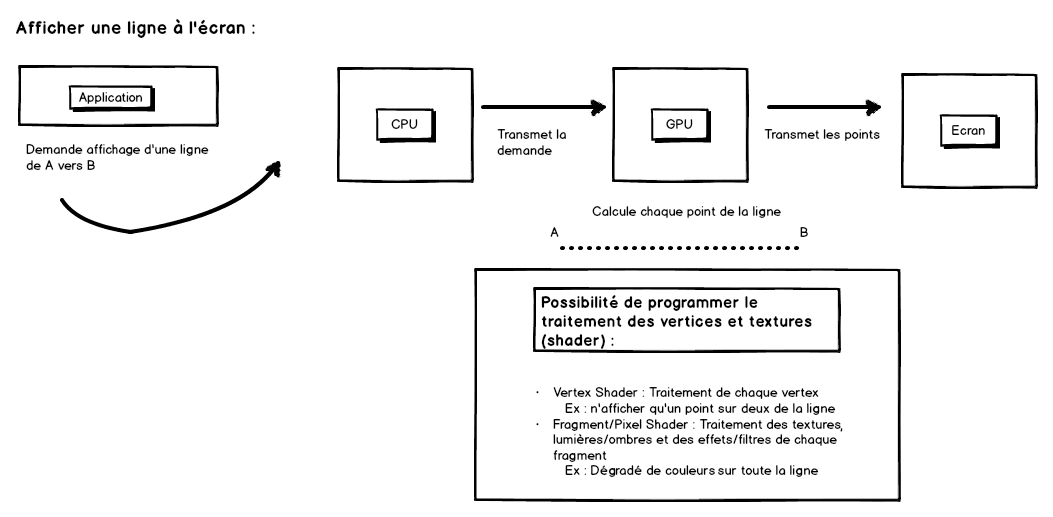
\includegraphics[width=15cm,height=8cm]{img/gpuRasterExemple.png}
\end{center}
Dans ce cas c'est le GPU qui va calculer tout les points de la ligne un par un. Etant optimisé pour effectuer de nombreux calculs en peu de temps. En effet, son architecture est faite de nombreux coeurs, certes moins puissants que ceux du CPU, mais cela lui permet d'effectuer beaucoup de calcul simultanément. \\
Le GPU envoyera ensuite les points à l'écran sous forme de pixel. \\\\
Avec les cartes graphiques modernes il est maintenant possible de programmer des parties de la carte graphique appelés shader (il en existe trois : les vertex, les geometriques et les pixels ou fragments). Ceux ci peuvent permettre par exemple d'appliquer un éclairage spécifique à notre ligne.
